\chapter{Technical Solution}

In this section an overview of the design, architecture and distinctive features of the solution is given. Then, technical decisions are explained.



\section{Design \& Architecture}

The architecture of this project is designed to meet the requirements discussed in section \ref{problem}. First, a bird's eye view is given on where this recommender framework fits into existing systems. Then, the internal architecture of the framework is explained. Finally, distinctive features of this framework are introduced.

\subsection{Serviceoriented Architecture (SOA)}

\begin{figure}[ht]
    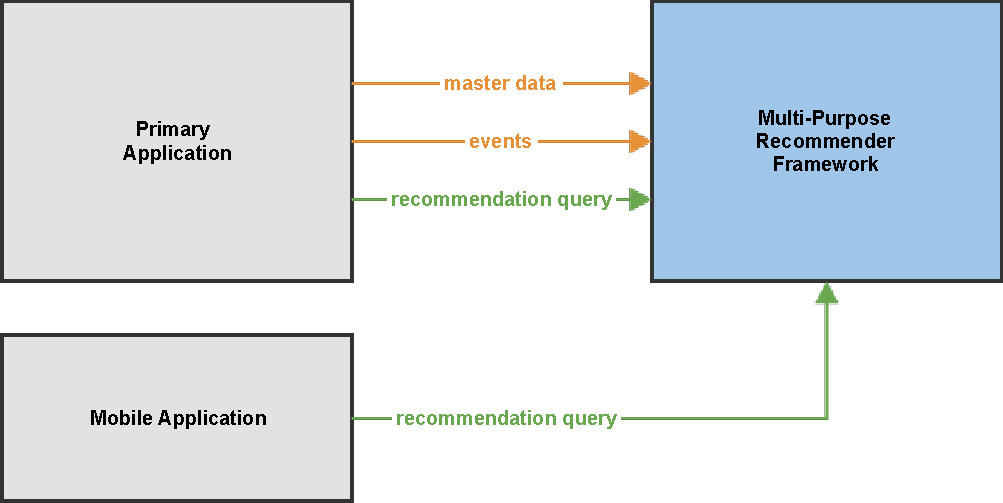
\includegraphics[width=0.7\textwidth,center]{solution/soa/soa.pdf}
    \caption[Service-Oriented Architecture (SOA)]{Service-Oriented Architecture (SOA). Orange arrows (\emph{master data} and \emph{event}) are \emph{notifications} whereas green arrows (\emph{recommendation query}) are \emph{queries} and expect a result.}
    \label{fig:soa}
\end{figure}

A \emph{service-oriented architecture (SOA)} is a software design pattern which is most suitable to meet the \emph{abstraction} requirement discussed in section \ref{problem-abstraction}. \emph{SOA} suggests to express features as services. This is true for features which are going to be available to other systems. Internal features are never to be exposed and allowed to be services. A \emph{service consumer} is a system using the service. \cite{erl08} identifies eight principles of \emph{SOA} of which I will elaborate:

\begin{description}
    \item[Standardised service contracts] is an expression of the service's purpose, capabilities and requirements -- such as mandatory parameters and data types. As long as the requirements are satisfied, the service agrees to fulfill its purpose.
    \item[Service loose coupling] makes sure that services have as few dependancies as possible.
    \item[Service abstraction] ensure that as much information as possible hidden and none except those described in the service contract are exposed.
    \item[Service reusability] assure that services are designed to be reused.
\end{description}

In figure \ref{fig:soa} a possible architecture of this project is shown. The framework is designed to serve more than one application or system component. The services accept requests from any source as long as they authorise with an access key. In the mentioned figure services are divided in two types -- \emph{notification} and \emph{query}. A \emph{notification} is a message relevant to the recommender framework and is simply acknowledged as received. A \emph{query} on the other hand expects a result. The framework will define three services:

\begin{description}
    \item[Master Data] enables service consumers to create, update or delete a data node in the framework. An identifier and type are mandatory fields. The service consumer is allowed to send any further features of the node which it thinks is relevant to the framework.
    \item[Event] accepts notifications about interactions or preferences between two or more nodes such as \emph{'X purchased Y and Z'}. The payload -- content of the message -- may contain a \emph{weight} which is a numeric value. It is useful for e.g. \emph{'X rated Y with 10'}.
    \item[Recommendation Query] requests recommendations for a specific recommendation model. The recommendation model identifier is mandatory. A node identifier and type are only mandatory if the model excepts it. This is the only service which expects a result.
\end{description}

The recommendation framework only expects incoming requests (\emph{push strategy}) and has no outgoing communication at all.

\subsection{Multilayered Architecture}
\label{sol-design-layer}

\begin{figure}[ht]
    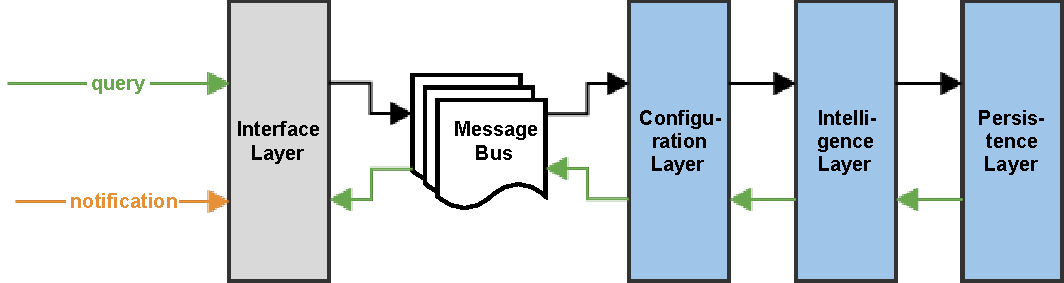
\includegraphics[width=\textwidth,center]{solution/layers/layers.pdf}
    \caption{Multilayered Architecture}
    \label{fig:ntier}
\end{figure}

A multi-layered architecture is a software design pattern for software programs which suggests separating functionality in responsibility layers. This is popular way of abstracting functionality within a system.

Strictly speaking, the framework is divided into two subsystems: the \emph{application programming interface (API)} and \emph{recommender ecosystem}. These subsystems are connected with a message bus. The motivation of this differentiation is of a technical rather than logical manner. The subsystems have different kind of technical requirements and this division allows me to use the most appropriate technology for each. Another side effect are the advantages of a message bus which allows me to group and prioritise messages. \emph{Recommendation queries} may be processed by a dedicated resource whereas \emph{event} messages may have higher priority -- and should be processed sooner -- than \emph{master data} messages. However this makes no difference to the responsibilities, and is therefore not further considered in the specification of layers.

\subsubsection{Interface Layer}

The interface layer is where services expose themselves to service consumers. Latter send requests to this layer. From a technical point of view this layer is implemented as an \emph{application programming interface (API)} via the \emph{hypertext transfer protocol (HTTP)} which is the foundation of data communication in the world wide web. The \emph{API} adopts the \emph{representational state transfer (REST)} style. An \emph{API} using \emph{REST} is called \emph{RESTful}. \citet{fielding00} -- who introduced \emph{REST} -- explains:

\begin{quotation}
    The name ``Representational State Transfer'' is intended to evoke an image of how a well-designed Web application behaves: a network of web pages (a virtual state-machine), where the user progresses through the application by selecting links (state transitions), resulting in the next page (representing the next state of the application) being transferred to the user and rendered for their use.
\end{quotation}

Two concepts of \emph{REST} are important to be understood: the use of \emph{uniform resource locator (URL)} and \emph{HTTP vocabulary}. The \emph{URL} provides a way to specify a resource -- in this case a service or node. The \emph{HTTP vocabulary} defines amongst others \emph{GET}, \emph{POST} and \emph{DELETE}. Combined a \emph{RESTful API} enables the access or modification of resources. E.g. to submit an event a \emph{POST} request to \emph{/events} is necessary. To delete a node with the identifier \emph{120} a \emph{DELETE} request to \emph{/nodes/120} is sufficient, whereas a \emph{GET} request to \emph{/recommendations/topseller} would return all recommendations for a recommendation model called \emph{topseller}.

This layer acts as \emph{service broker} and security agent at the same time. Latter is ensured by verifying the presence and correctness of an access key which is a random text. As a \emph{service broker} this layer validates the payload against mandatory fields and data types. Then, it offloads the message and submits it into the message bus for further processing. If the message is of the type \emph{notification} it acknowledges the request. If the message type is a \emph{query}, then it waits for a response from the message bus and returns that.

\subsubsection{Configuration Layer}
\subsubsection{Recommendation Layer}
\subsubsection{Persistance Layer}

\subsection{Distinctive Features}
\label{sol-design-features}

\subsubsection{Master Data}
\subsubsection{Event System}

\subsubsection{Recommender Plugin System}
\label{sol-feature-plugin}

\subsubsection{Recommendation Models}

%planning:
%- 500 words
%- figure
%- api layer
%- configuration layer
%- engine layer
%- event based
%- plugin system

\section{Implementation}

\subsection{Programming Languages \& Frameworks}

\subsubsection{JavaScript}
\subsubsection{Go}
\subsubsection{PHP}

\subsection{Databases}

\subsubsection{Neo4j}
\subsubsection{Redis}
\subsubsection{MySQL}

\subsection{Other Vendors}

\subsubsection{RabbitMQ}
\subsubsection{Git \& BitBucket}
